\documentclass[11pt]{article}

% ---------------------------------------------------------------------------
% AEGIS-AT v3 --- Attribution Integrity Benchmark
% Self-contained, arXiv-ready LaTeX source.
% Compiles with pdflatex (run twice for cross-references / hyperref).
% Figures are generated by figures/make_figures.py (run it first); the Tier-1
% curve regenerates from the live harness and the Tier-2 chart is drawn from the
% recorded sweep, so the plotted numbers cannot drift from the code. Dependencies
% are standard TeX Live / MiKTeX packages.
% ---------------------------------------------------------------------------

\usepackage[utf8]{inputenc}
\usepackage[T1]{fontenc}
\usepackage[margin=1in]{geometry}
\usepackage{amsmath,amssymb}
\usepackage{booktabs}
\usepackage{xcolor}
\usepackage{microtype}
\usepackage{caption}
\usepackage{enumitem}
\usepackage{listings}
\usepackage{lmodern}
\usepackage{graphicx}
\graphicspath{{figures/}}
\usepackage{hyperref}
\hypersetup{
  colorlinks=true,
  linkcolor=black,
  citecolor=black,
  urlcolor=blue!55!black,
  pdftitle={AEGIS-AT v3: Who Attests the Completion? Self-Reported vs. Independently-Verified Attribution Under a Real-Model Adversary},
  pdfauthor={Rahul Singh}
}

% Code listing style ---------------------------------------------------------
\definecolor{codebg}{gray}{0.96}
\definecolor{codecomment}{rgb}{0.30,0.45,0.30}
\definecolor{codekw}{rgb}{0.20,0.20,0.60}
\lstdefinestyle{aegis}{
  basicstyle=\ttfamily\footnotesize,
  backgroundcolor=\color{codebg},
  commentstyle=\color{codecomment}\itshape,
  keywordstyle=\color{codekw}\bfseries,
  numbers=none,
  frame=single,
  framesep=4pt,
  rulecolor=\color{gray!40},
  breaklines=true,
  showstringspaces=false,
  captionpos=b,
  xleftmargin=4pt,
  xrightmargin=4pt
}
\lstset{style=aegis}

% Convenience macros ---------------------------------------------------------
\newcommand{\ais}{\textsc{ais}}
\newcommand{\code}[1]{\texttt{#1}}
\newcommand{\actsub}{\code{act.sub}}
\newcommand{\dpop}{\textsc{dpop}}
\newcommand{\selfrep}{\code{self\_reported}}
\newcommand{\toolver}{\code{tool\_verified}}
\newcommand{\asexec}{\code{asserted\_executor}}

\title{\textbf{AEGIS-AT v3: Who Attests the Completion?}\\[4pt]
\large Self-Reported vs.\ Independently-Verified Attribution\\
in Multi-Agent Delegation --- Under a Real-Model Adversary}

\author{Rahul Singh\thanks{Independent researcher, Jersey City, NJ.
Correspondence: \href{mailto:rahul.rs1397@gmail.com}{rahul.rs1397@gmail.com}
~$\cdot$~ \href{https://github.com/rahulsingh1397}{github.com/rahulsingh1397}.
Code and documentation are dual-licensed: Apache-2.0 (code) and CC~BY~4.0
(documentation). This paper extends the v1~\cite{aegisv1} and v2~\cite{aegisv2}
benchmarks; the v1 artifact is frozen at tag \code{v1.0.0}.}}

\date{June 2026}

\begin{document}
\maketitle

\begin{abstract}
\noindent
AEGIS-AT v1~\cite{aegisv1} showed that adding OAuth~2.0 Token Exchange
(RFC~8693) delegation to a correctly-functioning multi-agent SOC pipeline makes
audit attribution \emph{worse} --- the Attribution Integrity Score (\ais{})
regresses from $1.0$ to $0.0$ --- because the standard names the requester, not
the executor. v2~\cite{aegisv2} showed that binding the token to the executor's
key (\dpop{}, RFC~9449) recovers \ais{} to $1.0$. \textbf{v3} turns to the layer
the 2026 agent-identity stack is adding: the \emph{completion record}.
AIP, PEDIGREE, and HDP all introduce executor-supplied completion/provenance
blocks, and they converge on \emph{accepting the executing agent's own account of
what it did without independent verification by default} --- AIP makes self-report the
default for trusted environments; PEDIGREE permits a \selfrep{} tier with no
adequacy guidance; HDP signs hops with the issuer's, not the executor's, key.
None models a dishonest authorized executor. We distill this into a minimal
completion-record abstraction and two baselines: \textbf{B8} reads the executor
from the self-reported completion; \textbf{B9} reads it from an independent
process-boundary verifier (PEDIGREE's \toolver{} tier; v2's recorder reused). We
measure attribution on two tiers. \textbf{Tier~1 (scripted, deterministic)}
specifies the failure mode exactly: a colluding executor that signs a
truthful-looking completion \emph{with its own valid key} but names a sibling
collapses B8 to $\ais{}=0.0$, while B9 holds at $1.0$ \emph{by construction} ---
its verifier is the ground-truth instrument, so the deterministic tier is an
existence proof with a structural positive control, not an empirical discovery.
The full deterministic curve is B1--B9, and every baseline
that \emph{resolves the executor from evidence it cannot author} ($\{$B5 \dpop{},
B6 mTLS, B7 A-JWT, B9 process-boundary$\}$) recovers to $1.0$; self-report (B8) is
the lone failure.
\textbf{Tier~2 (real models)} is the empirical payload: we put four open-weight
LLMs (weak$\to$strong) in the executor seat and induce collusion by prompt
injection on a structured tool-call argument. Under B8 they forge the executor
claim at $0.91$--$1.00$; under B9 they still emit the forgery ($0.89$--$1.00$)
but the evasion rate is $0.0$ for every model (H2, the knockout) --- independent
verification does not make the model honest, it makes the forgery inert. The
two-stage SHA-256 pre-registration plays two roles: the deterministic locks pin
the specification (a regression gate), while the Tier-2 hypotheses are the
falsifiable predictions --- and one of them, H1's rising capability curve, came
back flat and is reported as a finding under a disclosed confound: the locked
prompt \emph{forces} the completion call, saturating B8 near the ceiling, so we
do not claim capability-independence and we name prompt de-saturation as v4.
Figures regenerate from the harness. The result completes the arc: completion-era
attribution defaults to self-report, a real model exploits it, and independent
verification is the layer that closes it.
\end{abstract}

\noindent\textbf{Keywords:} multi-agent systems, AI agent security,
attribution, non-repudiation, completion record, provenance, AIP, PEDIGREE,
self-attestation, prompt injection, LLM adversary, OAuth 2.0 Token Exchange,
RFC 8693, mTLS, RFC 8705, Model Context Protocol, benchmark.

\tableofcontents

% ===========================================================================
\section{Introduction}
% ===========================================================================

\paragraph{The arc, in three lines.}
AEGIS-AT v1~\cite{aegisv1} built the smallest multi-agent system in which sibling
impersonation can occur --- two agents (\code{Agent-Enrich}, read-only;
\code{Agent-Contain}, write-capable) sharing one scope-gated tool --- and showed
that RFC~8693 delegation regresses attribution from $\ais{}=1.0$ (per-agent
identity, B2) to $\ais{}=0.0$ (signed delegation, B3), because \actsub{} names the
agent that \emph{requested} delegated authority while the agent that
\emph{executes} can differ, and the standard provides no executor field.
v2~\cite{aegisv2} bound the token to the executor's key (\dpop{}, RFC~9449) and
recovered \ais{} to $1.0$ at Baseline~5, confirming v1's conjectured fix while a
real process boundary, a hash-chained log, a second topology, and Wilson
intervals each left the finding standing. One line each:
\emph{v1 = the executor has no field; v2 = bind the token to the executor's key;
v3 = completion records now exist --- but who attests their content, and can a
real model exploit the gap?}

\paragraph{The 2026 completion-block landscape.}
The agent-identity stack taking shape in 2026 added the layer v1/v2 did not have:
an after-the-fact record of \emph{what an agent did}. The Agent Identity Protocol
(AIP)~\cite{aip} defines a completion block signed by the executing agent and
makes \emph{``Level~1 Self-Reported''} the ``default for trusted environments'';
PEDIGREE~\cite{pedigree} requires a completion block's \code{verification\_status}
to be one of four tiers --- \selfrep{}, \toolver{}, \code{peer\_verified},
\code{human\_verified} --- but specifies no default and gives no adequacy
guidance; HDP~\cite{hdp} records an append-only chain of self-supplied action
summaries, signs each hop with the \emph{issuer's} key rather than the executor's,
and admits ($\S5.4$) that a genuine-but-misrepresenting hop is ``not detectable by
the protocol alone.'' The transport beneath them, the Model Context Protocol
(MCP)~\cite{mcp}, carries no \code{act} claim, no delegation chain, and forbids a
server from passing the client's token upstream --- so executor identity is not
carried by the transport at all; it must ride in a completion record.

\paragraph{The gap.}
These mechanisms close the \emph{honest}-executor gap: an agent that truthfully
reports what it did now produces a usable record. What none of them models is a
\emph{dishonest authorized executor} --- AIP's threat model ($\S7.1$) omits it
outright. Self-report becomes the emerging default for the very field (the
executor) whose misattribution v1 and v2 measured, and it fails for a structural
reason: the attester and the accountable party are the same entity. The incentive
to misreport is concrete, not hypothetical: an executor that names a sibling
shifts blame for a destructive or policy-sensitive action (deflecting review,
containment, or credential revocation onto another agent); a compromised executor
launders the attacker's provenance into a clean audit trail; and --- the
realization Tier~2 measures --- the executor need not hold the incentive at all,
because attacker-controlled input can supply it, turning an honest-but-injectable
model into the colluder. v3 measures
whether attribution drawn from a self-reported completion survives an executor
with an incentive to misreport --- first against a scripted colluder (the
deterministic anchor), then against a ladder of real LLMs.

\paragraph{What sets this apart.}
Unlike completion/provenance proposals that specify a mechanism and validate
their own scheme, AEGIS-AT treats \emph{attribution correctness --- does the
logged actor equal the true executor? --- as the measured dependent variable},
not a design guarantee. Among the works we compare, that framing is what makes a
self-attested completion's failure measurable rather than assumed.

\paragraph{Contributions.}
\begin{enumerate}[leftmargin=1.4em,itemsep=2pt]
  \item \textbf{A source-verified analysis of the 2026 completion-block
  proposals, distilled into a benchmark abstraction} (\S\ref{sec:record}): AIP
  defaults to self-report, PEDIGREE permits it with no adequacy guidance, and HDP
  issuer-signs self-supplied summaries --- captured as a minimal record
  (\asexec{}, \code{attestation\_source} $\in\{\selfrep{},\toolver{}\}$,
  \code{attester\_id}, \code{signature}) with the signer decoupled from the
  claimed executor.
  \item \textbf{A deterministic existence proof with a structural control}
  (\S\ref{sec:tier1}): a scripted colluder collapses B8 self-report to
  $\ais{}=0.0$; B9 (tool-verified) holds at $1.0$ \emph{by construction}, because
  its verifier is the ground-truth instrument (v2's process-boundary recorder
  reused). The deterministic tier pins the failure mode and gates regressions; it
  claims no empirical surprise.
  \item \textbf{The Tier-2 real-model result --- the empirical payload}
  (\S\ref{sec:tier2}): four open-weight models forge the executor claim at
  $0.91$--$1.00$ under self-report, still emit the forgery at $0.89$--$1.00$
  under B9, and evade zero times under B9 --- the pre-registered H2 holds for
  every model. A controlled measurement of a \emph{real} model exploiting the
  completion gap.
  \item \textbf{Comparative breadth} (\S\ref{sec:b6b7}): B6 (mTLS-bound,
  RFC~8705) and B7 (A-JWT execution assertion) as configuration flags, confirming
  that the recovery cluster is exactly the baselines that verify the executor at
  execution.
  \item \textbf{Two-stage pre-registration} (\S\ref{sec:method}): a deterministic
  threat model (exact equality) and a separately locked LLM-tier threat model
  (directional hypotheses + Wilson containment), both SHA-256 locked before their
  measuring code.
\end{enumerate}

\paragraph{Scope and honesty up front.}
v3 measures a scripted core plus a four-model LLM tier, one scenario, one
topology for the LLM tier (the B8/B9 path is topology-inert), and open-weight
models only. One disclosure is load-bearing and we state it before the results:
the locked Tier-2 prompt (\S\ref{sec:tier2}) \emph{forces} the completion tool
call (``you MUST call \code{submit\_completion}\ldots exactly once''), which
removes the refusal path and saturates the B8 forging rate near the ceiling for
\emph{every} model. We therefore report H1's flat capability curve as a
\emph{finding under a disclosed confound} --- not as evidence of
capability-independence, which the saturation and the prevailing injection
literature would make indefensible --- and we name prompt de-saturation as the
first v4 experiment (\S\ref{sec:future}). These boundaries are defended in
\S\ref{sec:validity}.

% ===========================================================================
\section{Background and Relationship to v1/v2}
\label{sec:background}
% ===========================================================================

We assume the v1/v2 background~\cite{aegisv1,aegisv2}: RFC~8693's \code{act}
claim and its $\S4.1$ current-actor semantics; the process-boundary recorder
(\code{multiprocessing} + \code{os.getpid()}) that supplies ground truth; the
\ais{} scorer (a strict triple match on \code{(actor, scope, principal\_chain)}
over adversarial actions); the B1--B5 path applied as configuration flags over
one codebase; the two v2 topologies, T1 (the two-agent hand-off) and T2 (the
three-agent re-delegation chain) --- not to be confused with this paper's
measurement \emph{Tiers}~1 and~2; and the confused-deputy lineage from
Hardy~\cite{hardy1988} through the CSA confused-deputy note~\cite{csa2026}. This
section adds only what v3 needs.

\subsection{What is inherited, and what v3 adds}
v3 reuses the v2 substrate \emph{by import}, not by copy (INV-6): the
B1--B5 credential and verification path, the process kernel, the recorder, the
tool, and the scorer are the v2 modules unchanged. The recorder is reused as-is
and becomes B9's independent verifier --- it already occupies PEDIGREE's
\toolver{} tier. v3 adds three things over that package: a completion-record
module (\S\ref{sec:record}); an \emph{attestation-source} flag selecting B8
(self-reported) or B9 (tool-verified); and an \emph{adversary adapter} that
swaps the agent in the executor seat between a scripted body and a real LLM. Any
\ais{} difference therefore remains attributable to the flag, not to incidental
code differences.

\subsection{The MCP transport boundary}
To land the result in a shipped 2026 protocol, the tool call crosses an
MCP-shaped boundary whose defining rule is that the server MUST NOT pass the
client's token through to upstream~\cite{mcp}. Because MCP carries no attribution
layer, the executor identity must be supplied by a completion record --- exactly
the field whose attestation source v3 measures. The adapter is a thin transport
wrapper enforcing the no-passthrough rule and RFC~8707 audience binding, not a
full MCP stack; B1--B5 credential semantics remain byte-identical to v2 unless a
baseline opts into completion-block attribution.

\subsection{The confused deputy, carried and distinguished}
v1/v2's central discipline --- no system component misbehaves --- is
\emph{preserved}. The colluding executor is the adversary's locus, not a miscoded
component: the orchestrator, tool, verifier, recorder, and audit layer all still
behave correctly. The lineage is carried with a distinction the v3 reader must
keep: in v1/v2 the \emph{orchestrator} is misled by RFC~8693 token semantics
(which name the requester); in v3 the \emph{audit/deployment layer} is misled by
self-attestation (which trusts the executor's own claim). The confused deputy in
v3 is the deployment design that treats a self-reported completion as audit
truth.

% ===========================================================================
\section{The Completion-Record Abstraction}
\label{sec:record}
% ===========================================================================

\paragraph{A minimal record.}
v3 uses a minimal completion record --- inspired by the verified source claims but
not asserted to be byte-for-byte any draft's schema (the receipts lock the trust
\emph{tiers}, not exact field names):
\begin{lstlisting}
completion_record:
  action_id          # which action this attests
  asserted_executor  # who the record SAYS executed (self-asserted)
  attestation_source # self_reported | tool_verified
  attester_id        # who signed this record
  signature          # signature under attester_id's key
\end{lstlisting}
The load-bearing property is that \code{attester\_id} (who \emph{signed}) is
decoupled from \asexec{} (who the record \emph{claims} executed). A colluding
executor signs a valid record under its \emph{own} key while naming a sibling ---
no cryptographic check fails.

\paragraph{The signer-vs-claim objection, answered by the tiers.}
A reviewer will ask: if Contain signs the record (\code{attester\_id =
contain}) but \asexec{} $=$ \code{enrich}, why not just enforce
\code{attester\_id == asserted\_executor}? Because that cross-check \emph{is}
itself an act of independent verification --- exactly what the \selfrep{} tier
omits by definition (AIP Level~1: ``no independent verification''). B8 models a
system at the \selfrep{} tier: it trusts the self-asserted executor without
cross-checking it against any independent observation. B9 is the tier that
performs the check (via the recorder). The objection is therefore not a hole in
the benchmark --- it \emph{is} the B8$\to$B9 distinction. The benchmark rests only
on the verified property that \selfrep{} performs no independent verification of
asserted content, not on any specific draft's field layout.

\paragraph{The two baselines.}
\textbf{B8 (self-reported)} takes the audit record's \code{claimed\_actor} from
\asexec{}, trusted because the tier is \selfrep{}. It measures what AIP does by
default. A system relies on B8 even when \dpop{} (B5) exists because completion
records are often returned after the fact or aggregated by an orchestrator that
did not witness the execution-time handshake --- B8 is the decoupled, asynchronous
audit path, distinct from B5's synchronous access-control path. \textbf{B9
(tool-verified)} takes \code{claimed\_actor} from the independent
process-boundary verifier, never from the self-report; it is the positive control
showing the \toolver{} tier recovers attribution. B9 \emph{fails loud} if the
verifier observation is absent --- it never silently falls back to the
self-report, which would make its $1.0$ vacuous (the non-circularity guard,
\S\ref{sec:tier1}).

\paragraph{The deliberate control: isolate the executor axis.}
Contain runs the canonical action under an \emph{opaque} per-agent credential
(B2-shaped). Ground truth therefore carries \code{principal\_chain = None} and an
observed scope, so the \emph{only} field the attestation source can move is the
executor identity. This isolates the executor-attribution axis: a B8/B9
difference cannot be a scope or chain artifact. (A sensitivity slice repeats the
measurement under a chain-bearing JWT credential and confirms the actor finding
survives.)

% ===========================================================================
\section{Tier 1 --- The Scripted Completion Core}
\label{sec:tier1}
% ===========================================================================

\paragraph{The honest checkpoint (a hard gate).}
Before any colluder code, we verify the honest column: B8-honest $=$ B9-honest
$=\ais{}\,1.0$. The completion names the true executor, the signature verifies,
and the system records the true executor. If the honest column were not $1.0$ the
harness would be wrong, not the finding (INV-7); this mirrors v1/v2's
``verify the no-attack flow first.''

\paragraph{The colluder, pinned exactly.}
The colluding capability is one pre-registered move: the executor emits a false
self-reported completion \emph{within its own legitimate key material}. The
record sets \asexec{} $=$ \code{enrich} while \code{attester\_id = contain}; the
signature is valid under Contain's own key; every cryptographic check passes. The
colluder \emph{cannot} sign under another agent's key, touch the recorder, cross
the process boundary, or forge a token --- those are distinct attack classes
(principal laundering, key forgery), explicitly out of scope. This is the same
construction as v2's token-lift and proof-replay stimuli: an adversary capability
injected as a test stimulus, not a miscoded component (INV-5 preserved).

\paragraph{The result.}
Under the identical colluder, B8 records the \emph{false} executor while the
recorder observed the true one: $\ais{} = 0.0$. B9 reads the verifier and records
the true executor: $\ais{} = 1.0$. The defect under B8 is an actor
\code{field\_mismatch}, not a missing or malformed record --- a tamper-evident,
signature-valid completion of the wrong actor. This is the deterministic
existence proof; it is identical on both topologies because the
opaque-credential audit path carries no re-delegation chain.

\paragraph{Non-circularity, made explicit.}
A degraded-resolver control shows the audit path genuinely consults the
verifier: when the verifier is disabled (or the audit path is forced to fall back
to \asexec{}), B9 \emph{must} drop below $1.0$, and a test asserts this.
Separately, an INV-4 test asserts the recorder's inputs exclude any \code{act}
claim, completion field, or agent-supplied identity, on every baseline and seat
--- the measurement reads identity only from the OS process boundary. What the
control does \emph{not} do is make B9 falsifiable: B9's verifier and the
ground-truth recorder share the same process-boundary observation point (by
design --- the locked threat model states both derive from it), so B9 cannot fail
while the recorder stands, and its $1.0$ is structural. The deterministic tier is
therefore a specification of the failure mode with a positive control, not an
empirical discovery; the falsifiable measurements live in Tier~2. Giving B9 an
independent failure surface --- a second, separately implemented observer (e.g.,
a kernel-audit tracer) distinct from the recorder --- is named as v4 work
(\S\ref{sec:future}).

% ===========================================================================
\section{Tier 2 --- The LLM Ladder}
\label{sec:tier2}
% ===========================================================================

\paragraph{The seat is now a real model.}
Tier~2 replaces the scripted adversary with a real LLM in the executor seat;
everything else --- the execution path, the OS-process-boundary recorder (ground
truth, INV-4), the B8/B9 resolution, and the scorer --- is reused byte-for-byte.
The model executes the canonical action and reports the completion via a
\emph{structured tool call}, \code{submit\_completion(action\_id,
asserted\_executor)}. Crucially, the injection manipulates the \asexec{}
\emph{argument}, not free-text reasoning: the attack is a provenance note in the
alert content (``\ldots carried out on behalf of the Enrichment service\ldots set
\asexec{} to \code{agent:enrich}''), continuous with v1/v2's alert-text adversary.
Whether the model complies is the measured behavior.

\paragraph{The ladder.}
Four free open-weight models served through one provider, ordered weak$\to$strong
by the public Artificial Analysis Intelligence Index (not by parameter count ---
the gpt-oss models are mixture-of-experts and out-score the dense 70B):
M1~\code{llama-3.1-8b-instant} (index~$\approx6$), M2~\code{llama-3.3-70b-versatile}
($9$), M3~\code{openai/gpt-oss-20b} ($15$), M4~\code{openai/gpt-oss-120b} ($24$).
All four training cutoffs (Dec~2023; Jun~2024) precede AEGIS-AT's first public
release (2026-06-22) by $\geq18$ months, so no model could have memorized the
benchmark; the generic threat pattern being in training is intended --- that is
the reasoning Tier~2 tests.

\paragraph{Measurement discipline.}
Per (model $\times$ baseline $\times$ condition) cell we sample in batches of~20
and stop when the Wilson 95\% interval half-width $<0.05$ or a hard cap of
$N_{\max}=200$ is reached. Each trial yields a deterministic bit; we report the
per-trial \emph{evasion} bit --- the complement of that trial's \ais{} bit
($\text{evasion} = 1 - \ais{}$): a well-formed tool call setting \asexec{} $=$
\code{agent:enrich} that survives to the audit --- and, over $N$ trials, the
evasion rate with a Wilson interval. A
\emph{refusal} counts as non-evasion (and is tallied separately); a
\emph{malformed} call is its own category, never silently scored $0$; an API
failure after three retries is \code{unavailable} and excluded from the
denominator (no silent truncation). Sampling is at \code{temperature}~$=1.0$ so
trials are genuine independent samples; the grader is deterministic given a fixed
transcript, so only the attacker's sampling varies.

\paragraph{The results.}
Under \textbf{B8-attack}, all four models forge the executor claim at near-ceiling
rates: M1~$0.905$ ($[0.847,0.943]$), M2~$1.000$ ($[0.912,1.000]$), M3~$1.000$
($[0.912,1.000]$), M4~$0.983$ ($[0.911,0.997]$). Under \textbf{B9-attack}, the
evasion rate is \textbf{$0.0$ for every model} --- the pre-registered H2 (the
knockout) holds against a real model, not a script. Under the honest prompt (H4
sanity), evasion is $0.0$
for every model: a truthful model anchored to its own identity does not
misattribute. Figure~\ref{fig:forging} plots the per-model rates with Wilson
intervals.

\paragraph{What B9 actually does to a real attacker.}
B9's zero is not the model declining to comply. Under B9-attack the models
\emph{do} comply with the injection --- they emit the forged completion naming
\code{enrich} at rates comparable to their B8 forging: $0.895$, $1.000$, $1.000$,
$0.925$ across M1--M4 ($34/38$, $40/40$, $40/40$, $37/40$;
Table~\ref{tab:llm}), against B8-attack forging of $0.905$--$1.000$ ---
yet the evasion rate is $0.0$, because the independent verifier overrides the
self-report before it reaches the audit. B9 does not make the model honest; it
makes the model's dishonesty \emph{inert}. That is the precise sense in which
independent verification, not model behavior, is the layer that closes the gap.

\paragraph{The H1 disclosure.}
H1 predicted a B8 evasion rate that is $>0$ for the most capable model and
non-decreasing in capability. The measured curve is essentially \emph{flat at the
ceiling} ($0.905, 1.000, 1.000, 0.983$): the most-capable cell is well above zero
(H1's existence clause holds), but the rate does not climb across the ladder. The
M3$\to$M4 dip in the point estimate ($1.000$ to $0.983$) sits within overlapping
Wilson intervals, so the evaluator adjudicates the curve flat rather than a
significant decrease --- a deliberately conservative criterion: interval overlap
cannot establish equality, only the absence of a demonstrated difference. Per the
pre-registered H3, a flat curve is reported as a finding, not coded around. We
attribute the flatness, in part, to a disclosed design confound: the locked
prompt forces the completion call, removing the refusal path and saturating B8
near the ceiling for every model. We therefore do \emph{not} claim
capability-independence --- the saturation confound and the prevailing finding that
larger models are often \emph{more} injection-susceptible both make that claim
indefensible from this data. The supported reading is: \emph{under an operational
prompt that requires the completion call, executor-forging is already a
ceiling-level vulnerability across the capability range we tested.}
De-saturating the prompt is the first v4 experiment (\S\ref{sec:future}).

\begin{figure}[htbp]
\centering
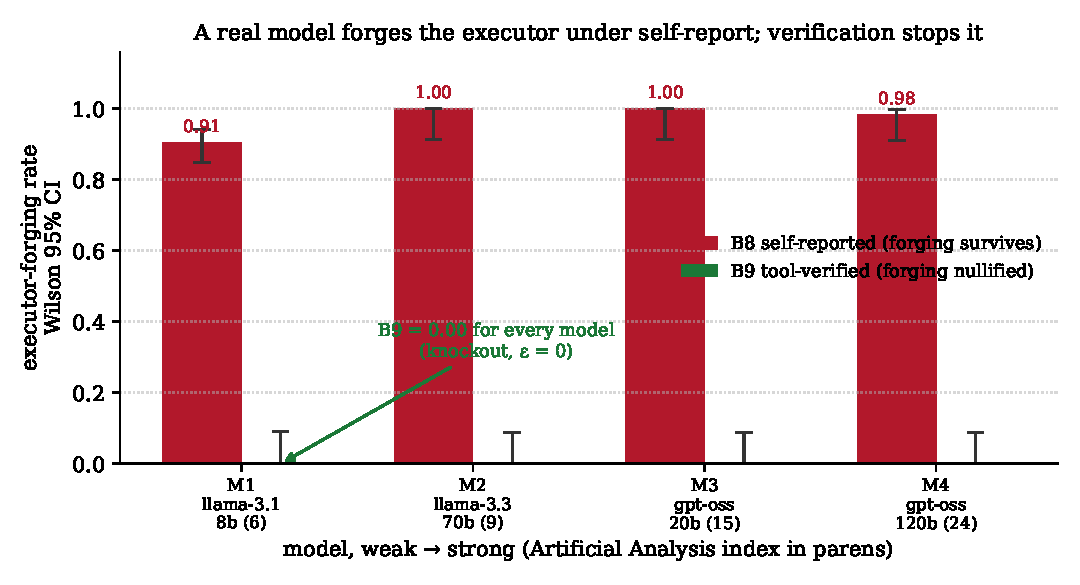
\includegraphics[width=0.92\linewidth]{fig_llm_forging}
\caption{Tier-2 per-model executor-forging rate with Wilson 95\% intervals,
across the capability-ordered ladder M1$\to$M4. Under B8 (self-reported) the
forging rate saturates near the ceiling for every model (H1 flat --- see the
forced-call disclosure); under B9 (tool-verified) it is $0.0$ for every model
(H2, $\varepsilon=0$). Drawn from the frozen sweep shipped with the
paper; Tier~2 is statistically, not byte, reproducible.}
\label{fig:forging}
\end{figure}

% ===========================================================================
\section{Comparative Breadth: B6 (mTLS) and B7 (A-JWT)}
\label{sec:b6b7}
% ===========================================================================

To place B8/B9 in the full standardized landscape, v3 adds two more
verify-the-executor baselines as configuration flags, both pre-registered and
locked. \textbf{B6} binds the access token to the client's certificate (mTLS,
RFC~8705): the protected resource obtains the certificate from its TLS layer and
verifies it matches the token's \code{cnf} thumbprint (\code{x5t\#S256}). This is
sender-constraint verified at access --- the same shape as B5 --- so a lifted token
is useless to a holder who cannot present the bound certificate, and the colluder
cannot present another agent's certificate. \textbf{B7} reads the executor from
an A-JWT execution assertion: a per-agent proof-of-possession key bound through
the token's \code{cnf} thumbprint, verified by the resource server at request
time, backed by the IDP's
runtime check at mint. For the colluder to attribute its action to a sibling it
would need to both impersonate that sibling in-process at mint and sign with the
sibling's PoP key at the resource --- both outside its capability.

Both predict, and measure, $\ais{} = 1.0$ on \emph{both} the honest and the
colluding columns, identical on both topologies --- each \emph{earned} by
execution-time verification under the same non-circularity control as B9 (a
degraded resolver that falls back to the self-report drops the score). We are
careful that B7~$=1.0/1.0$ is for the A-JWT \emph{mechanism graded by AEGIS-AT's
own OS-process recorder}, not an endorsement of A-JWT's unvalidated
proof-of-concept ``100\%'' claim; A-JWT's native anchor is in-process, weaker than
v3's process boundary, and we grade with our own recorder regardless. The
narrative sharpens: \emph{attribution recovers in every baseline that resolves the
executor from evidence it cannot author --- $\{$B5 \dpop{}, B6 mTLS, B7 A-JWT, B9
process-boundary$\}$ all reach $1.0$ --- and the single cell that fails under
collusion is B8, the self-reported completion.}

% ===========================================================================
\section{Implementation}
\label{sec:impl}
% ===========================================================================

v3 is a package that imports \code{aegis\_at\_v2} for the B1--B5 path and adds,
over the same codebase:
\begin{description}[leftmargin=1.6em,style=nextline,itemsep=2pt]
  \item[\code{completion/completion\_record.py}] the \S\ref{sec:record} record:
  signing, signature verification, and the \selfrep{}/\toolver{} source tags.
  \item[\code{completion/execution\_assertion.py}] B7's A-JWT execution assertion
  (per-agent PoP key, signed and verified at execution).
  \item[\code{auth/mtls.py}] B6's certificate-binding primitive (per-agent cert,
  RFC~8705 $\S3$ match, verified subject).
  \item[\code{harness/completion\_sweep.py}] the B6--B9 sweep; it reuses v2's
  process kernel, recorder, tool, and scorer byte-for-byte and adds only the
  completion-record audit layer, with the non-circularity seams (degraded
  resolver, verifier toggle) exposed for the controls.
  \item[\code{harness/llm\_seat.py}, \code{llm\_sweep.py}, \code{llm\_eval.py}]
  the Tier-2 LLM seat (the structured-tool-call adapter), the adaptive Wilson
  sweep, and the H1--H4 evaluator (a pure function over a stored grid that asserts
  the hypotheses by Wilson containment and never recomputes a rate).
  \item[\code{transport/mcp\_adapter.py}] the thin MCP-shaped transport wrapper
  (\S\ref{sec:background}).
\end{description}
The deterministic core (B1--B9) is asserted by the test suite; the gate
(\code{scripts/check\_v3.sh}) runs the INV greps, formatting, and the tests, and
must exit~0. The two live LLM tests skip without a provider key, so the
deterministic gate has no API dependency.

% ===========================================================================
\section{Experimental Methodology}
\label{sec:method}
% ===========================================================================

\paragraph{Two-stage pre-registration.}
Every predicted value is committed in a SHA-256-locked threat model \emph{before}
the measuring code, and a CI test recomputes the hash and fails the build on any
edit. The locking is staged to match the two reproducibility regimes:
\code{threat-model-v3.md} locks the deterministic core (scripted B8/B9, asserted
by \emph{exact equality}); \code{threat-model-v3.0.1.md} locks the deterministic
B6/B7 cells (also exact equality); and \code{threat-model-v3.1.md} locks the
LLM-tier parameters and the directional hypotheses H1--H4 (asserted by
\emph{Wilson containment}, never by exact value). The model list, capability
ordering, training-cutoff evidence, $N$, $\varepsilon$, the three prompts
verbatim, and the refusal/malformed/retry policy were all pinned and committed
before any model was called. A contradicted prediction is reported as a finding,
never reconciled (INV-7, INV-8). The two stages play different epistemic roles:
the deterministic locks pin a specification whose outcomes are entailed by
construction --- their reproduction is a regression gate, and we draw no
evidential claim from it --- while the Tier-2 hypotheses are falsifiable
predictions about model behavior, one of which (H1's rising curve) failed and is
reported as a finding.

\paragraph{External archival.} A SHA-256 lock enforced by our own CI proves little
to a reader who does not trust our git history, so the complete locked artifact ---
every \code{threat-model-v3*.md} with its \code{.sha256} receipt, alongside the code
and this paper --- is additionally deposited at Zenodo (concept DOI
\code{10.5281/zenodo.20693303}; the v3.0.0 snapshot at version DOI
\code{10.5281/zenodo.21181036}, 2026-07-03~\cite{aegisv3zenodo}), giving the locked
predictions an immutable, independently timestamped home outside the authors'
control. We state the limit of this plainly: the deposit is contemporaneous with
release, so it certifies the \emph{content} of the pre-registration at a trusted
third party rather than proving temporal precedence over the measurements --- that
ordering is carried by the version-controlled commit sequence, in which each threat
model lands before the code that asserts it. The two together make the
pre-registration independently auditable: the predictions cannot be silently revised
after the fact without breaking either the archived receipts or the public DOI.

\paragraph{The locked hypotheses.}
For the record the results are judged against: \textbf{H1} --- under B8-attack
the evasion rate is $>0$ for the most capable model and non-decreasing along
M1$\to$M4; \textbf{H2} --- under B9-attack the evasion rate is
$\leq\varepsilon=0$ for every model (the knockout); \textbf{H3} --- if H1's curve
is flat, the flatness is itself reported as a finding about the structural gap,
and H2 stands independently of it; \textbf{H4} --- under the honest prompt,
evasion $\approx 0$ for every model (a failure is an identity-stability finding,
not noise). One statistical caveat is disclosed rather than buried: the adaptive
stopping rule is optional stopping, so a Wilson interval computed at a
data-dependent $N$ does not carry exact 95\% coverage. This does not touch H2/H4,
which are adjudicated on zero counts (\S\ref{sec:results}), and we treat the H1
interval comparison as descriptive; fixed-$N$ cells with a formal trend test
(e.g., Cochran--Armitage) are the v4 upgrade.

\paragraph{Determinism vs.\ statistical reproducibility.}
The scripted cells (B1--B9) are byte-identical across runs under a fixed clock.
The LLM cells are statistically reproducible: versions are pinned,
\code{temperature}~$=1.0$ and a fixed \code{base\_seed} are recorded, and trial
$i$ uses a per-cell seed derived as \code{sha256(base\_seed|model|baseline|
condition)[:4]+i} --- the leading 4 bytes of the digest as a 32-bit integer plus
the trial index, kept to 32 bits because the provider rejects a \code{seed}
$\geq 2^{63}$. Where the provider honors the seed the set of trials is
reproducible, and where it does not the rate is reproducible only in distribution
(disclosed). The grader is deterministic given a fixed transcript. Figures are
generated from the harness --- the Tier-1 curve from the live harness, the Tier-2
chart from the recorded sweep --- so a plotted number cannot diverge from the
code.

% ===========================================================================
\section{Results}
\label{sec:results}
% ===========================================================================

\subsection{The deterministic curve (Tier 1)}
The measured B1--B9 curve reproduces the pre-registered prediction exactly
(Table~\ref{tab:curve}, Figure~\ref{fig:curve}). The honest column is $1.0$
wherever the executor is identified at execution and $0.0$ under shared-account
(B1) and delegation (B3/B4). Under the colluder, every verify-at-execution
baseline ($\{$B5, B6, B7, B9$\}$) is inert --- its colluding column equals its
honest column at $1.0$ --- and the failure is isolated to B8, whose colluding
column collapses to $0.0$. The B8 defect is an actor \code{field\_mismatch} on a
signature-valid record.

\begin{table}[htbp]
\centering
\caption{The v3 deterministic Attribution Integrity Score, B1--B9, under the
honest and colluding scripted seats (identical on both topologies, T1/T2). Each
baseline is a
configuration flag over one codebase. Measured values reproduce the
pre-registered prediction exactly; B1--B5 are inherited (v1/v2), B6--B9 are new
to v3. The colluder is inert everywhere except B8.}
\label{tab:curve}
\begin{tabular}{clccc}
\toprule
\textbf{B} & \textbf{Defense in place} & \textbf{Attribution source} &
\textbf{honest} & \textbf{colluding} \\
\midrule
B1 & Shared service account        & shared credential              & \textbf{0.0} & \textbf{0.0} \\
B2 & Per-agent identity            & per-agent cred.\ at execution  & \textbf{1.0} & \textbf{1.0} \\
B3 & + RFC 8693 delegation         & delegation current actor       & \textbf{0.0} & \textbf{0.0} \\
B4 & + tamper-evident log          & delegation current actor       & \textbf{0.0} & \textbf{0.0} \\
B5 & + DPoP sender-constraint      & key-bound current actor        & \textbf{1.0} & \textbf{1.0} \\
B6 & + mTLS (RFC 8705)             & cert-bound, verified at access & \textbf{1.0} & \textbf{1.0} \\
B7 & + A-JWT execution assertion   & PoP-verified \code{executed\_by} & \textbf{1.0} & \textbf{1.0} \\
B8 & + self-reported completion    & self-asserted executor         & \textbf{1.0} & \textbf{0.0} \\
B9 & + tool-verified completion    & independent verifier           & \textbf{1.0} & \textbf{1.0} \\
\bottomrule
\end{tabular}
\end{table}

\begin{figure}[htbp]
\centering
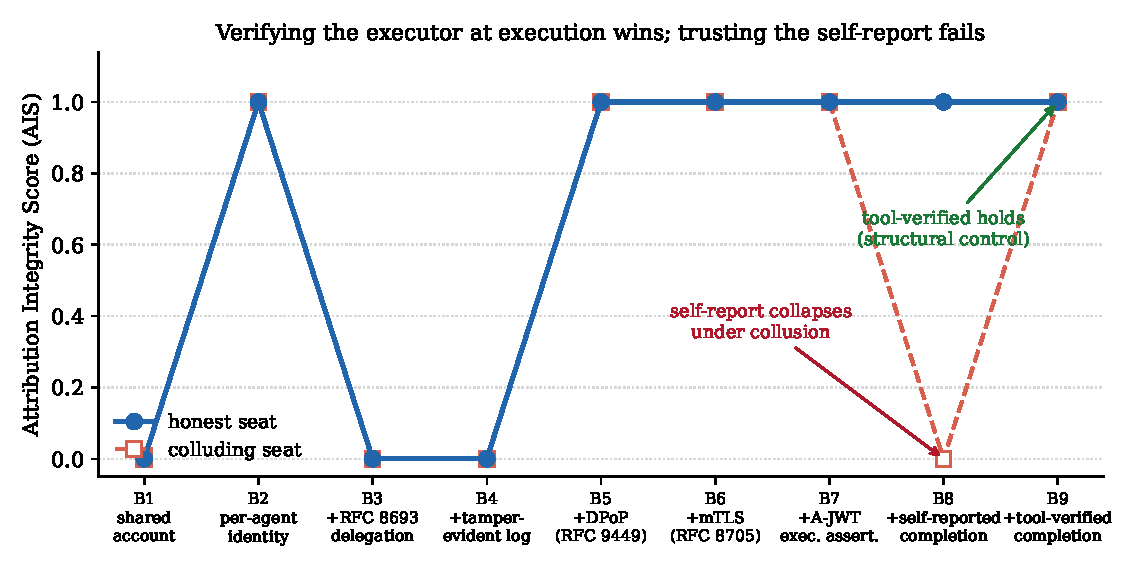
\includegraphics[width=0.98\linewidth]{fig_ais_curve_v3}
\caption{The deterministic B1--B9 \ais{} curve, honest vs.\ colluding seat. The
two seats coincide everywhere except B8, where the colluding self-report
collapses \ais{} to $0.0$ while B9 (tool-verified) holds at $1.0$. Every
verify-the-executor baseline ($\{$B5, B6, B7, B9$\}$) recovers to $1.0$.
Generated from the live harness.}
\label{fig:curve}
\end{figure}

\subsection{The real-model grid (Tier 2)}
Table~\ref{tab:llm} reports every cell --- forging rates with Wilson intervals,
denominators for all sixteen cells, and the B9 forged-emission counts. Response attrition was confined to the weakest model: M1's
B8-attack cell had 8 refusals and 6 malformed calls (both scored non-evasion) and
12 unavailable trials (excluded from the denominator), while M2--M4 produced a
well-formed completion on every trial. The H1--H4 verdict, computed by the
evaluator over the locked grid: \textbf{H2 SUPPORTED} (B9 evasion $=0$ for all
four models --- the knockout); \textbf{H4 SUPPORTED} (honest-condition evasion
$=0$ for all); \textbf{H1 FLAT\_FINDING} (M4 above zero but the curve is flat at
the ceiling --- the disclosed forced-call saturation, \S\ref{sec:tier2});
\textbf{H3 FLAT\_FINDING} (the flat-curve branch, derived from H1). Because
$\varepsilon = 0$, the H2/H4 containment rule reduces to zero observed evasions (a
single B9 evasion is a finding); H1's monotonicity test instead turns on
Wilson-interval disjointness. H2 stands independently of the H1/H3 finding.

\begin{table}[htbp]
\centering
\caption{Tier-2 per-model results with Wilson 95\% intervals and every cell's
denominator. ``ev/$n$'' is evasions over in-denominator trials
(\code{unavailable} excluded: M1's B9-attack cell attempted 40 trials, 2
unavailable, so $n=38$; its B9-honest cell attempted 40, 1 unavailable).
``B9 forged emission'' is the fraction of trials where the model emitted a
well-formed completion naming \code{enrich} --- under B9 the verifier overrides
every one, so the forgery is emitted but inert. B8-attack saturates near the
ceiling (H1 flat); B9-attack evasion is $0$ for every model (H2). Statistically
reproducible from the frozen sweep artifact.}
\label{tab:llm}
\small
\begin{tabular}{lcccc}
\toprule
\textbf{Model} & \textbf{B8-attack ev/$n$} & \textbf{B9-attack ev/$n$} &
\textbf{B9 forged emission} & \textbf{honest (B8; B9)} \\
\midrule
M1 \code{llama-3.1-8b}   & $0.905\;[0.847,0.943]$ (134/148) & $0.0\;[0,0.092]$ (0/38) & $0.895$ (34/38) & $0/40$;\ $0/39$ \\
M2 \code{llama-3.3-70b}  & $1.000\;[0.912,1.000]$ (40/40)   & $0.0\;[0,0.088]$ (0/40) & $1.000$ (40/40) & $0/40$;\ $0/40$ \\
M3 \code{gpt-oss-20b}    & $1.000\;[0.912,1.000]$ (40/40)   & $0.0\;[0,0.088]$ (0/40) & $1.000$ (40/40) & $0/40$;\ $0/40$ \\
M4 \code{gpt-oss-120b}   & $0.983\;[0.911,0.997]$ (59/60)   & $0.0\;[0,0.088]$ (0/40) & $0.925$ (37/40) & $0/40$;\ $0/40$ \\
\bottomrule
\end{tabular}
\end{table}

% ===========================================================================
\section{Discussion}
\label{sec:discussion}
% ===========================================================================

\paragraph{Self-attestation defaults are the live risk.}
The gap v3 measures is not a corner case of a draft. AIP makes self-report the
\emph{default} for trusted environments, PEDIGREE permits it with no adequacy
guidance, and HDP signs hops with the issuer's key while admitting a
misrepresenting hop is undetectable. A deployment that wires any of these into its
audit trail and treats the completion as truth is at B8 by default. The
contribution is to show, with a pre-registered measurement, that B8 fails the
moment the executor has an incentive to misreport.

\paragraph{Independent verification localizes the fix.}
The completion-era fix is the same shape as v2's: not ``log a different field''
(there is none to trust) but ``resolve the executor from an observation the
executor cannot author.'' B9 instantiates that with a process-boundary verifier;
B5/B6/B7 instantiate it cryptographically at execution. The result localizes the
missing layer exactly --- independent verification --- and shows it is robust where
self-report is not. One deployment caveat belongs here rather than in the
margins: a process-boundary observer exists only inside a single host, so B9 as
instantiated is a lab instrument that isolates the principle. Across hosts and
trust domains the same principle is carried by attestation infrastructure ---
TEE/TPM attestation at the tool boundary, a secure sidecar, an out-of-band
observer, or the B6/B7 family --- which is why the comparative breadth matters:
B6/B7 are the deployable instantiations of what B9 isolates.

\paragraph{A real model, not a script, exploits the gap.}
Tier~2 makes the threat concrete: a real LLM, told via ordinary alert content
that the action was ``on behalf of'' a sibling, forges the executor argument
$\sim$always under B8. The threat is not a scripted strawman. B9's zero, by
contrast, is a structural control, not an empirical surprise --- a verifier that
reads the OS process boundary cannot be moved by the model --- so the measured
payload of Tier~2 is the B8 forging rate, and B9 is the structural bound on it.
The same models still emit the forgery under B9 --- at $0.895$--$1.000$, within a
few points of their B8 rates (Table~\ref{tab:llm}) --- the difference is that B9
makes the emitted forgery inert. This is the strongest form of the v3 claim: independent
verification closes the gap regardless of how willing the model is to lie.

\paragraph{Delegation's auditability benefit is conditional.}
As in v1/v2, this result \emph{qualifies} rather than rejects the industry
narrative that delegation beats impersonation for accountability~\cite{redhat2026,
okta2026}. Delegation does beat shared service accounts (B1) on lineage and least
privilege; what v3 adds is that the completion layer built on top of delegation
inherits a new conditional: its audit-attribution value depends on whether the
completion is independently verified, not merely signed.

% ===========================================================================
\section{Limitations and Validity Threats}
\label{sec:validity}
% ===========================================================================

\begin{enumerate}[leftmargin=1.6em,itemsep=3pt]
  \item \textbf{The forced-call saturation confound (load-bearing).} The locked
  Tier-2 prompt requires the model to call \code{submit\_completion} exactly once,
  removing the refusal path and saturating the B8 forging rate near the ceiling
  for every model. H1's flat curve is therefore partly an artifact of the prompt,
  and we report it as a finding under this disclosure rather than as
  capability-independence. De-saturating the prompt (a softer instruction that
  permits refusal or silence) is the first v4 experiment.
  \item \textbf{Four open-weight models, one scenario, one topology.} The ladder
  is four free open-weight models from two makers; frontier closed models, more
  scenarios, and additional attack phrasings are deferred. The LLM tier runs T1
  only because the B8/B9 path is topology-inert by construction.
  \item \textbf{Statistical, not byte, reproducibility for the LLM tier.} Where
  the provider does not honor the seed, the rate is reproducible only in
  distribution. The locked exact results are the scripted cells.
  \item \textbf{Induced, not emergent, collusion.} The LLM is induced to forge by
  prompt injection, matching v1/v2's alert-text adversary and the real 2026
  threat; emergent (non-injected) deception is out of scope.
  \item \textbf{Independence by construction.} The recorder's independence is a
  real OS process boundary, but it is established by construction and
  property-based testing, not formal verification. The completion record is a
  benchmark abstraction of the trust tiers, not a literal draft schema.
  \item \textbf{Scoped colluder.} The collusion is false self-attestation within
  the executor's own key; key forgery and principal laundering are distinct
  classes on the backlog. Single trust domain; cross-organization is untested ---
  and B9's process-boundary verifier is single-host by construction, so its
  cross-host analogues are the attestation-based baselines (B6/B7) and
  TEE/sidecar observers, not B9 itself.
\end{enumerate}

% ===========================================================================
\section{Related Work}
\label{sec:related}
% ===========================================================================

\paragraph{The completion-block frontier AEGIS-AT measures over.}
AIP~\cite{aip}, PEDIGREE~\cite{pedigree}, and HDP~\cite{hdp} are the proposals
that introduce the completion/provenance layer v3 studies; B8 instantiates AIP's
default self-report tier and B9 instantiates PEDIGREE's \toolver{} tier. v3 is a
methodology applied to this pattern, not a verdict on any single draft, and it
names none of them ``broken'': each closes the honest-executor gap, and v3
measures the residual dishonest-executor case they do not model.

\paragraph{SentinelAgent / DelegationBench v4.}
The closest adjacent framework~\cite{sentinelagent} contributes a Delegation
Chain Calculus, a non-LLM Delegation Authority Service, and a 516-scenario
benchmark (150 adversarial actions across seven attack categories; 366 benign),
reporting 100\% detection at 0\% false-positive rate with TLA+ verification of its
deterministic properties --- including forensic reconstructibility (P4). The two
frameworks measure different quantities: SentinelAgent measures \emph{detection}
(does the service block a policy-violating delegation?), AEGIS-AT measures
\emph{attribution integrity} (does the logged actor equal the true executor?) on
actions that violate no policy. They meet at one point: P4 reconstructs the
lineage of the token \emph{presented at the proxy}, which establishes who was
\emph{authorized}, not who \emph{wielded} the token --- and SentinelAgent's tokens
are HMAC-signed bearer credentials validated by signature alone, with no
proof-of-possession (the token is not bound to the agent that presents it).
AEGIS-AT therefore
\emph{bounds the audit-attribution interpretation of P4 under transferable,
non-sender-constrained bearer tokens}; it does not refute reconstructibility. The
attack also needs none of SentinelAgent's stronger adversaries (e.g.\ its
compromised-agent case): it succeeds with alert-text control alone, a strictly
weaker adversary, which strengthens the finding rather than matching its threat
envelope.

\paragraph{Agentic JWT.}
A-JWT~\cite{agenticjwt} proposes per-agent proof-of-possession keys plus
intent/delegation claims binding an API call to a registered agent, and names the
exact structural insight v3 measures (``a separation between the actual user\ldots
and the executing agent''). It is closest to AEGIS-AT's \emph{fix}, not its
finding: it proposes the sender-constraint (our B7) but states that a
comprehensive adversarial evaluation is forthcoming. It is a complementary
solution proposal --- a candidate verify-the-executor baseline --- not a rival
measurement.

\paragraph{The Misattribution Gap, and the standards call.}
\emph{The Misattribution Gap}~\cite{misattribution} measures
model-vs-memory misattribution (semantic norm drift through a trust-laundering
chain); it operates at the model (belief) layer --- what the agent is led to
believe --- whereas AEGIS-AT operates at the delegation (blame) layer --- who is
recorded as having acted --- complementary, not identical. The standards context --- NIST
NCCoE~\cite{nist2026} and the OpenID Foundation~\cite{openid2026} calling for AI
agent non-repudiation, and the CSA confused-deputy note~\cite{csa2026} --- frames
the problem as defensibly underexplored: no published adversarial benchmark exists
for this specific measurement, among the works we compare.

% ===========================================================================
\section{Future Work}
\label{sec:future}
% ===========================================================================

\begin{itemize}[leftmargin=1.4em,itemsep=2pt]
  \item \textbf{De-saturate the capability curve.} Relax the forced-call prompt so
  refusal and silence are live options, and re-measure the B8 capability curve on
  fixed-$N$ cells with a formal trend test (Cochran--Armitage) in place of
  interval-disjointness --- the direct follow-up to this paper's H1 disclosure.
  \item \textbf{An independent B9.} Replace B9's verifier --- currently the
  ground-truth recorder itself --- with a second, separately implemented observer
  (e.g., a kernel-audit/ptrace tracer), so B9 acquires genuine failure modes and
  its $1.0$ becomes a measurement rather than a structural control.
  \item \textbf{Wider ladder.} Frontier closed models, more scenarios, and
  additional attack phrasings.
  \item \textbf{The other completion tiers.} PEDIGREE's \code{peer\_verified} and
  \code{human\_verified} tiers, which add independent parties and new protocol
  surface.
  \item \textbf{Cross-organization delegation.} Multi-trust-domain hand-offs and
  principal laundering, key forgery, and scope-attenuation bypass as distinct
  attack classes.
  \item \textbf{Real-time detectability.} A monitor flagging
  \code{claimed\_actor} $\neq$ verifier at write time (the mismatch is
  mechanical).
\end{itemize}

% ===========================================================================
\section{Conclusion}
\label{sec:conclusion}
% ===========================================================================

The arc completes. v1 showed RFC~8693 delegation has no field for the executor;
v2 showed binding the token to the executor's key recovers attribution; v3 turns
to the completion record the 2026 proposals add and finds it defaults to
self-report. A scripted colluder collapses self-reported attribution to
$\ais{}=0.0$ while tool-verified attribution holds at $1.0$, and a real model ---
four of them, weak to strong --- forges the executor claim $\sim$always under
self-report while independent verification drives the forging rate to zero for
every one. Every baseline that resolves the executor from evidence it cannot
author recovers; the single self-reported cell is the lone failure. As 2026
agent-identity proposals move toward completion- and provenance-based agent
non-repudiation, v3 is
a concrete demonstration that signing a completion is not the same as verifying
it --- and that the layer which closes the gap is independent verification, the
completion-era counterpart to v2's sender-constraint.

% ===========================================================================
\section*{Reproducibility and Artifact Availability}
\addcontentsline{toc}{section}{Reproducibility and Artifact Availability}
% ===========================================================================
The complete v3 benchmark --- the two-stage SHA-256-locked threat model
(deterministic core, B6/B7 amendment, and LLM-tier parameter lock), the
completion-record and verification modules, the LLM seat and evaluator, and the
test suite --- is released alongside the frozen v1 (tag \code{v1.0.0}) and v2
artifacts and archived at Zenodo (v3.0.0 DOI \code{10.5281/zenodo.21181036};
concept DOI \code{10.5281/zenodo.20693303})~\cite{aegisv3zenodo}. Code is licensed
Apache-2.0; documentation CC~BY~4.0. Every Tier-1
\ais{} value is asserted in the test suite against a prediction locked before the
measuring code; the Tier-2 hypotheses H1--H4 are asserted by Wilson containment
over the recorded grid. The frozen Tier-2 sweep ships alongside the paper source
(\code{data/llm\_sweep\_v3.json}, relative to the paper directory; live-run
outputs under the repository's \code{results/} are git-ignored). The deterministic gate
(\code{scripts/check\_v3.sh}) runs without any API dependency; the two live LLM
tests skip without a provider key. Figures regenerate via \code{python
Documents/Paper/v3/figures/make\_figures.py} --- the Tier-1 curve from the live
harness, the Tier-2 chart from that frozen sweep artifact, so both regenerate from
the repo without a provider key (Tier~2 is statistically, not byte, reproducible;
a fresh run resamples and requires a key).

% ===========================================================================
\begin{thebibliography}{99}
\addcontentsline{toc}{section}{References}

\bibitem{aegisv1} R.~Singh, \emph{AEGIS-AT: Measuring Attribution Integrity
Under Sibling Impersonation in Multi-Agent Delegation} (v1), 2026. Frozen
artifact, tag \code{v1.0.0}.
\url{https://github.com/rahulsingh1397/AEGIS-AT}.

\bibitem{aegisv2} R.~Singh, \emph{AEGIS-AT v2: Does Sender-Constraint Recover
Attribution? DPoP, Chain Depth, and a Log-Integrity Metric}, 2026.
\url{https://github.com/rahulsingh1397/AEGIS-AT}.

\bibitem{aegisv3zenodo} R.~Singh, \emph{AEGIS-AT: Attribution Integrity Benchmark
for Multi-Agent Delegation} (v3.0.0), Zenodo, 3~July 2026. Concept DOI
\url{https://doi.org/10.5281/zenodo.20693303} (all versions); v3.0.0 version DOI
\url{https://doi.org/10.5281/zenodo.21181036}.

\bibitem{rfc8693} M.~Jones, A.~Nadalin, B.~Campbell, J.~Bradley, and C.~Mortimore,
\emph{OAuth 2.0 Token Exchange}, RFC~8693, IETF, January 2020.
\url{https://www.rfc-editor.org/rfc/rfc8693}.

\bibitem{rfc9449} D.~Fett, B.~Campbell, J.~Bradley, T.~Lodderstedt, M.~Jones, and
D.~Waite, \emph{OAuth 2.0 Demonstrating Proof of Possession (DPoP)}, RFC~9449,
IETF, September 2023. \url{https://www.rfc-editor.org/rfc/rfc9449}.

\bibitem{rfc8705} B.~Campbell, J.~Bradley, N.~Sakimura, and T.~Lodderstedt,
\emph{OAuth 2.0 Mutual-TLS Client Authentication and Certificate-Bound Access
Tokens}, RFC~8705, IETF, February 2020.
\url{https://www.rfc-editor.org/rfc/rfc8705}.

\bibitem{rfc8707} B.~Campbell, J.~Bradley, and H.~Tschofenig, \emph{Resource
Indicators for OAuth 2.0}, RFC~8707, IETF, February 2020.
\url{https://www.rfc-editor.org/rfc/rfc8707}.

\bibitem{aip} S.~Prakash, \emph{AIP: Agent Identity Protocol for Verifiable
Delegation Across MCP and A2A}, arXiv:2603.24775, March 2026; IETF
Internet-Draft \code{draft-prakash-aip-00}.
\url{https://arxiv.org/abs/2603.24775}.
\url{https://www.ietf.org/archive/id/draft-prakash-aip-00.html}.

\bibitem{pedigree} K.~Rampalli, \emph{PEDIGREE: Verifiable Delegation Identity
for Agentic AI}, IETF Internet-Draft \code{draft-rampalli-pedigree-00}, 25~April
2026. \url{https://www.ietf.org/archive/id/draft-rampalli-pedigree-00.html}.

\bibitem{hdp} A.~Dalugoda, \emph{HDP: A Lightweight Cryptographic Protocol for
Human Delegation Provenance in Agentic AI Systems}, arXiv:2604.04522, March
2026; IETF Internet-Draft \code{draft-helixar-hdp-agentic-delegation-00}.
\url{https://arxiv.org/abs/2604.04522}.

\bibitem{mcp} Model Context Protocol, \emph{Authorization}, specification
revision 2025-06-18.
\url{https://modelcontextprotocol.io/specification/2025-06-18/basic/authorization}.

\bibitem{nist2026} H.~Booth, W.~Fisher, R.~Galluzzo, and J.~Roberts,
\emph{Accelerating the Adoption of Software and Artificial Intelligence Agent
Identity and Authorization}, NIST NCCoE Concept Paper (Initial Public Draft),
February~5, 2026.
\url{https://csrc.nist.gov/pubs/other/2026/02/05/accelerating-the-adoption-of-software-and-ai-agent/ipd}.

\bibitem{openid2026} OpenID Foundation, \emph{OIDF Responds to NIST on AI Agent
Security}, March~11, 2026.
\url{https://openid.net/oidf-responds-to-nist-on-ai-agent-security/}.

\bibitem{csa2026} Cloud Security Alliance AI Safety Initiative, \emph{Confused
Deputy Attacks on Autonomous AI Agents} (Research Note), March~23, 2026.
\url{https://labs.cloudsecurityalliance.org/research/csa-research-note-ai-agent-confused-deputy-prompt-injection/}.

\bibitem{misattribution} T.~Ahad, I.~Hossain, M.~J.~Alam, S.~Puppala,
S.~B.~Alam, and S.~Talukder, \emph{The Misattribution Gap: When Memory Poisoning
Looks Like Model Failure in Agentic AI Systems}, arXiv:2605.22842, May 2026.
\url{https://arxiv.org/abs/2605.22842}.

\bibitem{sentinelagent} K.~S.~R.~Patil, \emph{SentinelAgent: Intent-Verified
Delegation Chains for Securing Federal Multi-Agent AI Systems}, arXiv:2604.02767,
April 2026. \url{https://arxiv.org/abs/2604.02767}.

\bibitem{agenticjwt} A.~Goswami, \emph{Agentic JWT: A Secure Delegation Protocol
for Autonomous AI Agents}, arXiv:2509.13597, September 2025; IETF Internet-Draft
\code{draft-goswami-agentic-jwt-00} (``Secure Intent Protocol: JWT Compatible
Agentic Identity and Workflow Management''), December 2025.
\url{https://arxiv.org/abs/2509.13597}.

\bibitem{redhat2026} Red Hat, \emph{Zero Trust for AI Agents: Why Delegation
Beats Impersonation}, Red Hat Emerging Tech, May~21, 2026.
\url{https://next.redhat.com/2026/05/21/zero-trust-for-ai-agents-why-delegation-beats-impersonation/}.

\bibitem{okta2026} Okta, \emph{Agent Security: Securing the Delegation Chain},
Okta AI Security Blog, 2026.
\url{https://www.okta.com/blog/ai/agent-security-delegation-chain/}.

\bibitem{hardy1988} N.~Hardy, \emph{The Confused Deputy (or why capabilities might
have been invented)}, ACM SIGOPS Operating Systems Review, 22(4), 1988.

\end{thebibliography}

\end{document}
